\chapter{Introduction}
\label{introductio}

This chapter will highlight the working environment, the project background as well as its aim.
 
\section{Working environment}
 
\subsection{University of Aalen}
The university of Aalen was founded in 1962 and by now is one of the leading university's of applied sciences in Germany. It has a focus in technical and economic research and has approximately 6000 students.
The University is located in Aalen, a smaller city in the south of Germany. The University has ongoing cooperations with many companies in the region such as Zeiss, Mapal and Trumpf. Further, Aalen University has international cooperations with 136 other Universities.\cite{Aalen}
 
\subsection{Workshop}
The practical part of this project was carried out in my home workshop. The workshop has tools for basic metal work, wood work, a 3D-Printing as well as some tools for the development of electronics. Further, equipment for welding, conventional milling and turning is available.
 
 
\section{Project background}
The mechatronic project is fixed part of the masters program "System Engineering" at Aalen University. It is supposed to cover both practical and theoretical work for solving a mechatronic problem.\\
In the theoretical part of the project, the problem needs to be split in smaller individual issues. In the next step, solutions for each of the issues need to be found by thoroughly analyzing the requirements of the projects.\\
In the practical part of the project, the previously discovered issues and the solutions for it are supposed to be translated and tested to their functionality in practice.\\
This development process can be summarized in the so called V-Modell. The V-Modell is shown in \ref{V-Model Complete}.
 
\begin{figure}
    \begin{center}
    \includegraphics[width=12cm]{Pictures/VModelComplete.png}
    \caption[V-Model Complete]{V-Model}
    \label{V-Model Complete}
    \end{center}
\end{figure}
 
The motivation and idea of this project were founded by my interest in metal work as well as online sources about similar projects.\cite{CloughELS}
 
\subsection{Aim of study}
The aim of this project is to add the Electronic Lead screw system to the Emco Compact 8 mini Lathe (see Appendix \ref{AppendixListOfCompanies}) in a way that is reversible. This is important in order to remain the value of the lathe. Further, the ELS system is supposed to be an addition that speeds up and simplifies the manual operation of the lathe by replacing the manual gearbox with electronics. For this reason, it is not planned to add servos to the other axis of the lathe in the future. Both, the Lathe as well as the Gearbox that is going to be replaced are shown in Figure \ref{AimLathe}.
 
 

\begin{figure}
    \begin{center}
    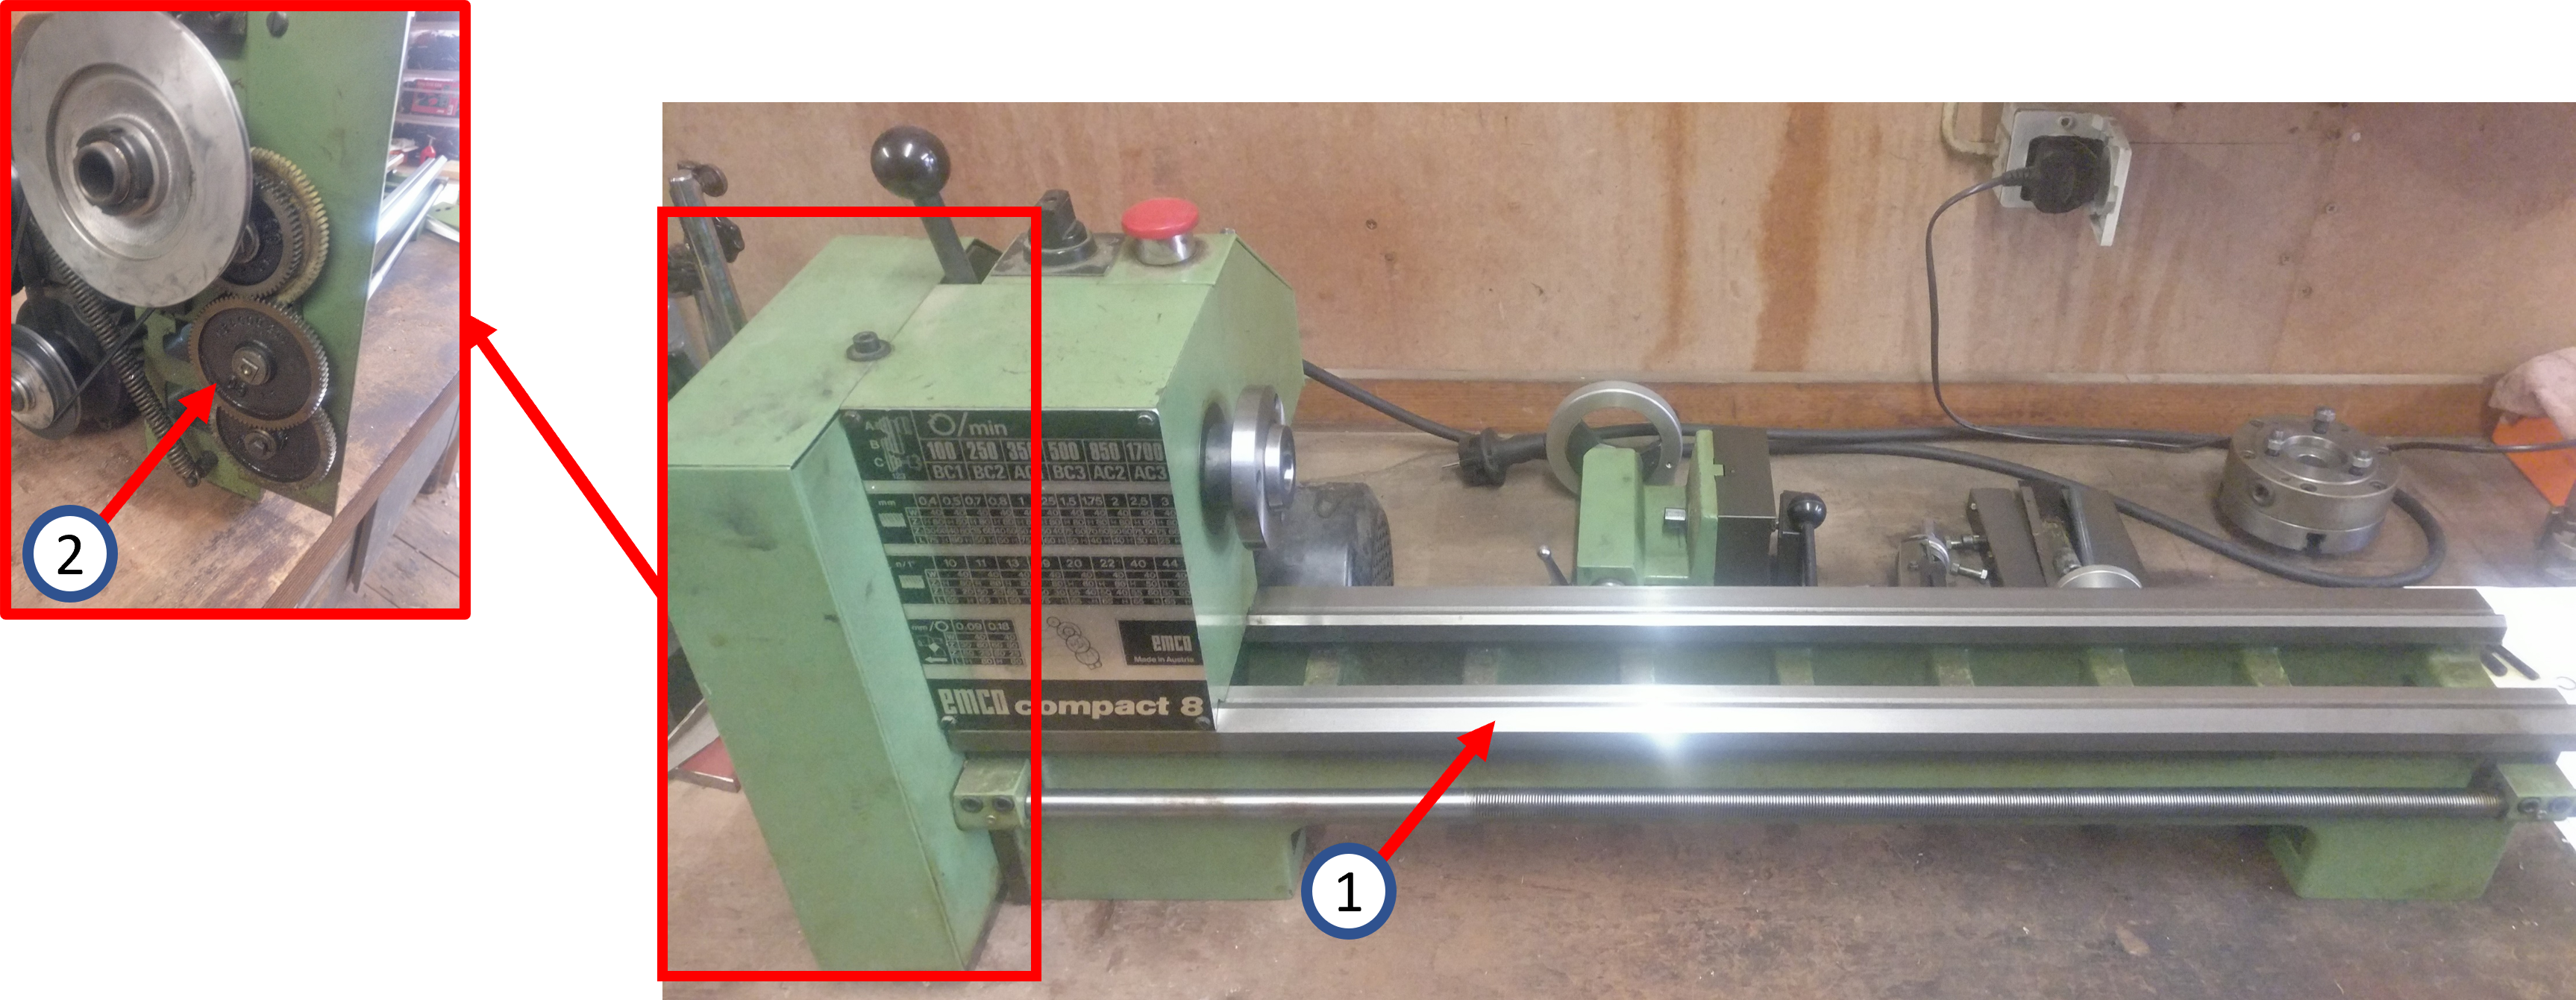
\includegraphics[width=12cm]{Pictures/AimLathe.png}
    \caption[Image of the Emco Compact 8 and the manual gearbox]{Image of the Emco Compact 8 and the manual gearbox; 1 - Emco Compact 8, 2 - Manual gearbox}
    \label{AimLathe}
    \end{center}
\end{figure}



